\chapter{Introduction}

\section{Motivation}

\yerotherpblack is an \textbf{Enterprise Resource Planing (ERP)}
software--system that aims 'effectiveness' and 'simplicity',
compared to other high ranked ERP software--systems
(e.g.: \sageerp, \saperp, etc.).

We chose to design and implement \yerotherpblack as
a \thickclient software--system because of the
following reasons:

\begin{enumerate}[1.]

	\item the implementation language \cplusplus
		offers much flexibility (use of macro, 
		multiple inheritance, etc.)
	
	\item the drawback of the multiple inheritance
		feature of \cplusplus is it can sometimes
		be very difficult to build it using "\gplusplus" !
		
	\item the availability of \texttt{'WHAT YOU SEE IS WHAT YOU GET'}
		(\wy) tools for fast and useful
		user interface design (e.g.: \qtdesigner~\cite{qtdesigner:2020},
		\ministudio~\cite{miniStudio:2020}, etc.)
		
	\item the low number of logical software architecture
		layer ($2$) involved with the operation
		of a \thickclient software--system,	as opposed
		to a \webbrowserbased software--system
		(with at least a $4$ layers in its 
		logical software architecture ).
	
\end{enumerate}


\section{Thick--Client VS Web--Browser--based
	Software--System Architecture}


\begin{table*}[!htbp]
\centering
\resizebox{\textwidth}{!}{%to fit the table within the text width
\begin{tabular}{cccc} 

\multicolumn{1}{c}{}										&
Thick--client application \mycheckmark{yerothColorBlue}	& 
Web--browser--based application								\\ \hline

business code								&
		\yerothvert{user interface}			&						
		\yerothrouge{application server}	\\ \hline
		
co--related software--systems		&
		\yerothvert{$1$ (DBMS)}		&						
		\yerothrouge{at least $3$ (DBMS, web~/~application server)}	\\ \hline
						
number of logical layers									&
		\yerothvert{$2$ (client and data)}					&						
		\yerothrouge{$4$ (client, presentation, logic, and data)}\\ \hline
				
rapid prototyping (\wy tools)		&
		\yerothvert{yes}			&						
		\yerothrouge{very limited}	\\ \hline				
				
software security vulnerability										&
		\yerothvert{low ($1$ programming language)}					&					
		\yerothrouge{high (\emph{several} programming languages)}	\\ \hline

user interface 														&
		\yerothvert{all computers (GUI with \emph{BUSINESS CODE})}	&						
		\yerothvert{all computers (web--browser)}					\\ 		


\end{tabular}}
\caption{Thick--client application VS Web--browser--based application.\\}
\label{tab:thickclient-application-againts-webbrowserbased-application}
\end{table*}

\begin{center}
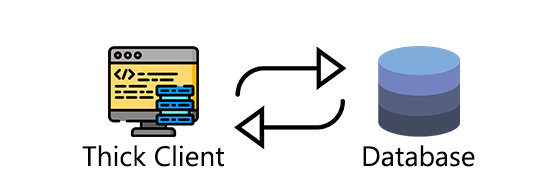
\includegraphics[scale=0.52]{images/yeroth-thickclient-application-two-tier-architecture.png}
\captionof{figure}{$2$--layers logical 
architecture of \thickclient software--system 
(Image copied from \cite{securityboulevarddotcom:2020}).}
\label{fig:yeroth-thickclient-application-two-tier-architecture}
\end{center}

Figure~\ref{fig:yeroth-thickclient-application-two-tier-architecture}
illustrates an example of a \thickclient
software--system with a $2$--layers
logical architecture.

\begin{center}
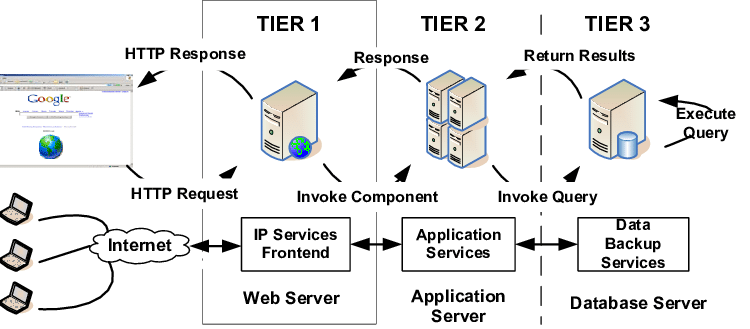
\includegraphics[scale=0.39]{images/yeroth-three-tier-architecture.png}
\captionof{figure}{$4$--layers logical architecture
of \webbrowserbased software--system
(Image copied from \cite{trevor:2006}).}
\label{fig:yeroth-three-tier-architecture}
\end{center}

Figure~\ref{fig:yeroth-three-tier-architecture}
illustrates an example of a \webbrowserbased
software--system with a $3$--layers
logical architecture.

Table~\ref{tab:thickclient-application-againts-webbrowserbased-application}
compares \thickclient software--systems against
\webbrowserbased software--systems.
